 \chapter{Goals and approaches}\label{chap:goals}
The overall goal of this research is to design an efficient software update management system for both SA-WSN and MA-WSN. The efficiency here means that the system has to satisfy the resource constraints of WSNs, with a lower power consumption. To achieve the main goal, each major component in the software update management framework needs to be modified with novel techniques and algorithms to address the challenges described above. The abstracted framework is shown in Figure~\ref{fig:framework}.

\begin{figure}[htbp]
	\centering
		\includegraphics[scale=0.45]{figures/framework.eps}
	\caption{The abstracted framework.}
	\label{fig:framework}
\end{figure}

The components that require modifications are:
\textbf{Compiler}
Instead of using a traditional compiler, an update-conscious compilation (UCC) technique is deserved in the WSN software update. Besides the code performance, the code similarity with another code image needs to be considered as well. 
The proposed UCC technique involves UCC register allocation (UCC-RA) and UCC data allocation (UCC-DA).

\textbf{Patch generator}
A patch generator is then used to summarizes the binary level code differences in a highly condensed style. Instead of explicitly listing the instruction level differences in the patch, the code structure changes, such as the register assignment switch and memory layout changes, are addressed directly in the patch script in order to reduce the patch size. 

\textbf{Distribution Protocol}
As mentioned in Chapter~\ref{chap:intro}, I divide the WSN {\it software update} into two circumstances, {\it software upgrade} and {\it software switch}.
While doing {\it software upgrade}, I adopted the existing code distribution protocol Deluge~\cite{deluge} to propagate the software upgrade patches from the sink node to the sensors that need upgrade. 
For \textit{software switch}, I proposed a multi-cast based code distribution protocol to let the sensors download the wanted binary code from the neighboring nodes that have the code image in memory. A dynamically updated routing table is used to guide the routing of the code requests to reach the source nodes.


The design goals of the software update framework are:
\begin{itemize}
\item reduce the overall energy consumption in software update.
\item reduced overall time consumption in software update.
\item the code dissemination protocol and the code retrieval algorithm run on the sensors have to obey the sensor network constrains, discussed in chapter~\ref{chap:intro}.
\end{itemize}

The design goals of this proposal will be accomplished by completing each individual components and integrating them as a complete framework. The design approaches of each framework component are discussed as below.

